\documentclass[tikz,12pt]{standalone}

\usepackage{amsmath,amsfonts,amssymb,amsthm}
\usepackage{mathptmx}
\usepackage{tikz}
\usepackage{xcolor}

\definecolor{tblue}{RGB}{25,102,243} % blue
\definecolor{bole}{rgb}{0.8, 0.0, 0.0} % brown
\usetikzlibrary{patterns}
\usetikzlibrary{arrows}

\begin{document}

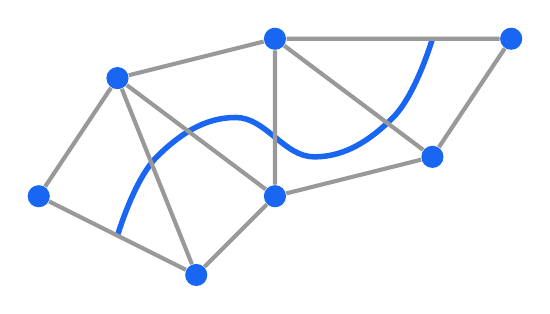
\begin{tikzpicture}
\tikzstyle{nodeBlue} = [
  shape=circle, 
  minimum size=8pt,
  inner sep=0pt,
  fill = tblue
]
\tikzstyle{tedge} = [
  draw = black!40,
  line width = 1.5,
]

\draw [line width = 2, tblue]  plot[smooth, tension=.7] coordinates {
  (-1,-1.5) (-0.5,-0.5) (0.5,0) (1.5,-0.5) (2.5,0) (3,1)
};

\node[nodeBlue] (v1) at (0,-2) {};
\node[nodeBlue] (v2) at (-2,-1) {};
\node[nodeBlue] (v3) at (-1,0.5) {};
\node[nodeBlue] (v4) at (1,-1) {};
\node[nodeBlue] (v5) at (1,1) {};
\node[nodeBlue] (v6) at (3,-0.5) {};
\node[nodeBlue] (v7) at (4,1) {};

\draw[tedge] (v1) -- (v2) -- (v3) -- (v1) -- (v4) -- (v3) -- (v5) -- (v4) -- (v6) -- (v5) -- (v7) -- (v6);

\end{tikzpicture}

\end{document}